\documentclass{beamer}

\usepackage{svg}
\usepackage{tikz}
\usetheme{CambridgeUS}

%%%%%%%%%%%%%%%%%%%%%%%%%%
%%% --- TITLE PAGE --- %%%
%%%%%%%%%%%%%%%%%%%%%%%%%%

\title[BMSSP]{Breaking the Sorting Barrier for Directed Single-Source Shortest
Paths}

\subtitle{Ein Blick über die wissenschaftliche Arbeit}
\author[Tascan, Durie, Lackner]{B. Tascan, B. Durie, S. Lackner}
\date[WAP 2025/26]{\today}

\setbeamertemplate{title page}{
    \begin{center}
        {\usebeamerfont{title}\inserttitle\par}
        \vspace{0.3cm}
        {\usebeamerfont{subtitle}\insertsubtitle\par}
        \vspace{0.5cm}
        {\usebeamerfont{author}\insertauthor\par}
        \vspace{0.3cm}
        {\usebeamerfont{institute}\insertinstitute\par}
        \vspace{0.3cm}
        {\usebeamerfont{date}\insertdate\par}
        \vspace{0.50cm}
        %\includegraphics[width=5.5cm]{logo1.png}
    \end{center}
}

%%%%%%%%%%%%%%%%%%%%%%%%%%
%%% --- INSTITUTE --- %%%
%%%%%%%%%%%%%%%%%%%%%%%%%%

%\institute[PLUS]{
%    FB Informatik\\
%    Universität Salzburg
%}

%%%%%%%%%%%%%%%%%%%%%%%%%%%%%
%%% --- OTHER CONFIGS --- %%%
%%%%%%%%%%%%%%%%%%%%%%%%%%%%%

\setbeamertemplate{navigation symbols}{}

\AtBeginSubsection[]
{
  \begin{frame}
    %\frametitle{Verzeichnis}
    \tableofcontents[
        currentsection
    ]
  \end{frame}
}

%%%%%%%%%%%%%%%%%%%%%%%%%%%%%
%%% --- CUSTOMISE END --- %%%
%%%%%%%%%%%%%%%%%%%%%%%%%%%%%
\begin{document}

\begin{frame}
    \titlepage
\end{frame}

%\logo{
%  \begin{minipage}{1cm}
%    %\hfill
%    \includegraphics[height=1cm]{logo2.png}
%  \end{minipage}
%}

\begin{frame}{Verzeichnis}
    \tableofcontents
\end{frame}

\section{Einführung}

\subsection{SSSP Algorithmen}

\begin{frame}{SSSP Algorithmen}
    \begin{itemize}
        \item<1-> Single-Source Shortest Path Algorithmen (SSSP's) 
        \begin{itemize}
            \item<2-> Input: ein Graph $G$ und ein Startknoten $s$
            \item<2-> Output: Der kürzeste Pfad von s nach alle anderen Knoten
        \end{itemize}
        \item<3-> Verwendet meistens für:
        \begin{itemize}
            \item<3-> GPS-Navigation
            \item<3-> Network Routing
            \item<3-> Video-Spiele
        \end{itemize}
        \item<4-> Es gibt zwei SSSP Algorithmen, die uns interessieren:
        \begin{itemize}
            \item<4-> Dijkstra's Algorithmus,
            \item<4-> Bellman-Ford's Algorithmus
        \end{itemize}
    \end{itemize}
\end{frame}

\begin{frame}{kleiner Exkurs}
    \begin{itemize}
        \item<1-> Greedy Algorithmen:
        
        Algorithmen, die in jedem Schritt die lokalbeste Entscheidung treffen. 
        \item<2-> Frontier:
        
        Die Menge bereits abgeschlossener Knoten, 
        durch die jeder noch nicht gefundene kürzeste Pfad zwingend hindurchführen muss.

        \item<3-> Ein Knoten relaxieren:
        
        Alle Kanten von einem Knoten checken und die Distanzen verbessern, 
        falls ein kürzerer Pfad entstanden ist.
    \end{itemize}
\end{frame}

\subsubsection{Dijkstra}

\begin{frame}{Dijkstra}
    \begin{itemize}
        \item<1-> Von Edsger W. Dijkstra im Jahr 1959 publiziert.
        \item<2-> 66 Jahre lang der asymptotisch schnellste Algorithmus
        \item<3-> Dijkstra's ist ein \textit{Greedy Algorithmus}.
    \end{itemize}
\end{frame}

\begin{frame}{Dijkstra}
  \begin{columns}
    \begin{column}{0.55\textwidth}
      \begin{itemize}
        \item min-Prioritätswarteschlange zur Auswahl des nächsten Knotens
        \item $\mathcal{O}(m + n \color{red}\log n\color{black})$
        \item 
      \end{itemize}
    \end{column}

    \begin{column}{0.51\textwidth}
      \centering
        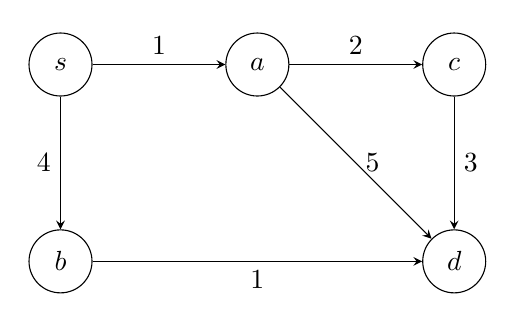
\begin{tikzpicture}[
            ->,
            >=stealth,
            node distance=2.5cm,
            vertex/.style={circle, draw, minimum size=8mm},
            every edge/.style={draw}
        ]

        % Nodes
        \node[vertex] (s) {$s$};
        \node[vertex] (a) [right of=s] {$a$};
        \node[vertex] (b) [below of=s] {$b$};
        \node[vertex] (c) [right of=a] {$c$};
        \node[vertex] (d) [below of=c] {$d$};

        % Edges (all non-negative!)
        \path
        (s) edge node[above] {1} (a)
        (s) edge node[left] {4} (b)
        (a) edge node[above] {2} (c)
        (a) edge node[right] {5} (d)
        (b) edge node[below] {1} (d)
        (c) edge node[right] {3} (d);

        \end{tikzpicture}
    \end{column}
  \end{columns}
\end{frame}

\subsubsection{Bellman-Ford}

\begin{frame}{Bellman-Ford}
    \begin{itemize}
        \item<1-> Unabhängig von Bellman (1958) und Ford (1956) entwickelt 
        \item<2-> Klassischer SSSP-Algorithmus für gerichtete Graphen
        \item<3-> Funktioniert mit \textit{negativen Kantengewichten}
        \item<4-> {Kein} Greedy-Algorithmus
    \end{itemize}
\end{frame}

\begin{frame}{Bellman-Ford}
    \begin{itemize}
        \item<1-> Initialisiere Distanzen
        \item<2-> Wiederhole $n-1$ Mal:
        \begin{itemize}
            \item<3-> Relaxiere \textbf{alle Kanten}
        \end{itemize}
        \item<4-> Optional: zusätzliche Runde erkennt negative Zyklen
        \item<5-> Jede Iteration erweitert bekannte kürzeste Pfade um genau eine Kante
    \end{itemize}
\end{frame}

\begin{frame}{Bellman-Ford}
    \begin{columns}
        \begin{column}{0.55\textwidth}
            \begin{itemize}
                \item Laufzeit: $\mathcal{O}(n \cdot m)$
                \item Deutlich langsamer als Dijkstra
                \item Dafür sehr robust
            \end{itemize}
        \end{column}

        \begin{column}{0.51\textwidth}
            \centering
            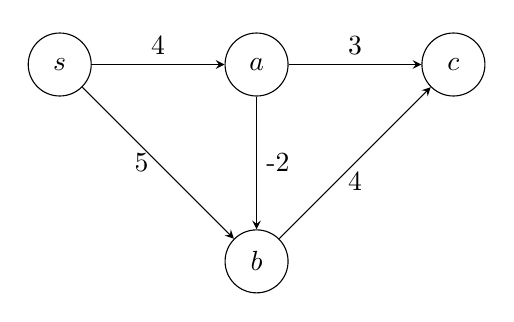
\begin{tikzpicture}[
                ->,
                >=stealth,
                node distance=2.5cm,
                vertex/.style={circle, draw, minimum size=8mm},
                every edge/.style={draw}
                ]
            % Nodes
            \node[vertex] (s) {$s$};
            \node[vertex] (a) [right of=s] {$a$};
            \node[vertex] (b) [below of=a] {$b$};
            \node[vertex] (c) [right of=a] {$c$};
            % Edges
            \path
            (s) edge node[above] {4} (a)
            (s) edge node[left] {5} (b)
            (a) edge node[right] {-2} (b)
            (a) edge node[above] {3} (c)
            (b) edge node[below] {4} (c);

            \end{tikzpicture}
        \end{column}
    \end{columns}
\end{frame}


%BMSSP%
\section{Bounded Multi-Source Shortest Path}
\subsection{Der Algorithmus}

%Einleitung%
\begin{frame}{Der Algorithmus - Einleitung}
    \begin{columns}[c, onlytextwidth]
        \begin{column}{.5\textwidth}
            \begin{itemize}[<+->]
                \item Dijkstra in $\mathcal{O}(m + n\log n)$
                \item Sortierbarriere $\Omega(n\log n)$
            \end{itemize}
        \end{column}

        \begin{column}{.4\textwidth}
            \centering
            \fbox{
                \includesvg[width=\linewidth, height=0.7\textheight, keepaspectratio]{divide-and-conquer-1}
            }
        \end{column}

        \begin{column}{.1\textwidth}
        \end{column}
    \end{columns}
\end{frame}

\begin{frame}{Der Algorithmus - Lösungsansatz}
    Sortierbarriere umgehen durch:
    \vspace{0.6cm}
    
    \begin{itemize}[<+->]
        \item \textbf{Eigene Datenstruktur} \\ 
        Ermöglicht effizientes \textit{Bucketing}, verhindert Sortierung
        \vspace{0.4cm}
        
        \item \textbf{Pivoting} \\ 
        Reduziert den Rechenaufwand
        \vspace{0.4cm}
        
        \item \textbf{Divide \& Conquer} \\ 
        Mindert die Problemgröße durch Rekursion
    \end{itemize}
\end{frame}

%Divide and conquer%
\begin{frame}{Der Algorithmus - Divide \& Conquer}
    \begin{tikzpicture}[remember picture, overlay]
        \node at ([yshift=-0.5cm]current page.center) {
            \fbox{%
                \includesvg[height=0.8\textheight]{divide-and-conquer-1}%
            }
        };
    \end{tikzpicture}
\end{frame}


\begin{frame}{Der Algorithmus - Divide \& Conquer}
    \begin{tikzpicture}[remember picture, overlay]
        \node at ([yshift=-0.5cm]current page.center) {
            \fbox{%
                \includesvg[height=0.8\textheight]{divide-and-conquer-2}
            }
        };
        \node[
            fill=white,
            draw=beamer@blendedblue,
            thick, 
            rounded corners, 
            inner sep=8pt,
            opacity=0.9,
            text opacity=1,
            anchor=north east
        ] at ([xshift=-0.5cm, yshift=-1.8cm]current page.north east) {
            $2^t \text{ Partitionen mit } t = \lfloor \log^{2/3} n \rfloor$
        };

    \end{tikzpicture}
\end{frame}

\begin{frame}{Der Algorithmus - Divide \& Conquer}
    \begin{tikzpicture}[remember picture, overlay]
        \node at ([yshift=-0.5cm]current page.center) {
            \includesvg[height=0.8\textheight]{divide-and-conquer-3}%
        };
    \end{tikzpicture}
\end{frame}

\begin{frame}{Der Algorithmus - Divide \& Conquer}
    \begin{tikzpicture}[remember picture, overlay]
        \node at ([yshift=-0.5cm]current page.center) {
            \fbox{%
                \includesvg[height=0.8\textheight]{divide-and-conquer-part-2}%
            }
        };
        \node[
            fill=white,
            draw=beamer@blendedblue,
            thick, 
            rounded corners, 
            inner sep=8pt,
            opacity=0.9,
            text opacity=1,
            anchor=north east
        ] at ([xshift=-0.5cm, yshift=-2.5cm]current page.north east) {
            $\lceil(\log n) /  t \rceil \text{ Rekursionen}$
        };
    \end{tikzpicture}
\end{frame}

\begin{frame}{Der Algorithmus - Divide \& Conquer}
    Wozu das ganze?
    \vspace{0.6cm}
    ist notwendiges Hilfsmittel für:
    \begin{itemize}
        \item \textbf{BMSSP} \\ 
        funktioniert nur dank Abgrenzungen
        \vspace{0.4cm}
        \item \textbf{Pivots} \\ 
        erlaubt schnelle Auswahl von wichtigen Knoten
    \end{itemize}
\end{frame}

%BMSSP
\begin{frame}{Der Algorithmus - BMSSP}
    \begin{tikzpicture}[remember picture, overlay]
        \node at ([yshift=-0.5cm]current page.center) {
            \fbox{%
                \includesvg[height=0.6\textheight]{bmssp-1}%
            }
        };
    \end{tikzpicture}
\end{frame}

\begin{frame}{Der Algorithmus - BMSSP}
    \begin{tikzpicture}[remember picture, overlay]
        \node at ([yshift=-0.5cm]current page.center) {
            \fbox{%
                \includesvg[height=0.6\textheight]{bmssp-2}%
            }
        };
    \end{tikzpicture}
\end{frame}

\begin{frame}{Der Algorithmus - BMSSP}
    \begin{tikzpicture}[remember picture, overlay]
        \node at ([yshift=-0.5cm]current page.center) {
            \fbox{%
                \includesvg[height=0.6\textheight]{bmssp-3}%
            }
        };
    \end{tikzpicture}
\end{frame}

\begin{frame}{Der Algorithmus - BMSSP}
    \begin{tikzpicture}[remember picture, overlay]
        \node at ([yshift=-0.5cm]current page.center) {
            \fbox{%
                \includesvg[height=0.6\textheight]{bmssp-4}%
            }
        };
    \end{tikzpicture}
\end{frame}

\begin{frame}{Der Algorithmus - BMSSP}
    \begin{tikzpicture}[remember picture, overlay]
        \node at ([yshift=-0.5cm]current page.center) {
            \fbox{%
                \includesvg[height=0.6\textheight]{bmssp-4}%
            }
        };
        \node[
            fill=white,
            draw=beamer@blendedblue,
            thick, 
            rounded corners, 
            inner sep=8pt,
            opacity=0.9,
            text opacity=1,
            anchor=north east
        ] at ([xshift=-0.5cm, yshift=-2cm]current page.north east) {
            Konkrete Suche via Mini-Dijkstra über $k$-Schritte
        };
    \end{tikzpicture}
\end{frame}

\begin{frame}{Der Algorithmus - BMSSP}
    Wozu das ganze?
    \vspace{0.6cm}
    \begin{itemize}
        \item \textbf{Sortierbarriere} \\ 
        Ermöglicht Umgehung der $\Omega(n\log n)$ Schranke dank Bucketing
    \end{itemize}
\end{frame}

%Pivots%
\begin{frame}{Der Algorithmus - Pivots}
    \begin{tikzpicture}[remember picture, overlay]
        \node at ([yshift=-0.5cm]current page.center) {
            \fbox{%
                \includesvg[height=0.8\textheight]{pivots-1}%
            }
        };
        \node[
            fill=white,
            draw=beamer@blendedblue,
            thick, 
            rounded corners, 
            inner sep=8pt,
            opacity=0.9,
            text opacity=1,
            anchor=north east
        ] at ([xshift=-0.25cm, yshift=-1.25cm]current page.north east) {
            $k$ Bellman-Ford Schritte
        };
    \end{tikzpicture}
\end{frame}

\begin{frame}{Der Algorithmus - Pivots}
    \begin{tikzpicture}[remember picture, overlay]
        \node at ([yshift=-0.5cm]current page.center) {
            \fbox{%
                \includesvg[height=0.8\textheight]{pivots-2}%
            }
        };
        \node[
            fill=white,
            draw=beamer@blendedblue,
            thick, 
            rounded corners, 
            inner sep=8pt,
            opacity=0.9,
            text opacity=1,
            anchor=north east
        ] at ([xshift=-0.25cm, yshift=-1.25cm]current page.north east) {
            \text{Markiere Knoten anhand nähester Quelle}
        };
    \end{tikzpicture}
\end{frame}

\begin{frame}{Der Algorithmus - Pivots}
    \begin{tikzpicture}[remember picture, overlay]
        \node at ([yshift=-0.5cm]current page.center) {
            \fbox{%
                \includesvg[height=0.8\textheight]{pivots-2}%
            }
        };
        \node[
            fill=white,
            draw=beamer@blendedblue,
            thick, 
            rounded corners, 
            inner sep=8pt,
            opacity=0.9,
            text opacity=1,
            anchor=north east
        ] at ([xshift=-0.25cm, yshift=-1.25cm]current page.north east) {
            Bäume mit mindestens $k$ Knoten $\Rightarrow$ Pivots
        };
    \end{tikzpicture}
\end{frame}

\begin{frame}{Der Algorithmus - Pivots}
    \begin{tikzpicture}[remember picture, overlay]
        \node at ([yshift=-0.5cm]current page.center) {
            \fbox{%
                \includesvg[height=0.8\textheight]{pivots-2}%
            }
        };
        \node[
            fill=white,
            draw=beamer@blendedblue,
            thick, 
            rounded corners, 
            inner sep=8pt,
            opacity=0.9,
            text opacity=1,
            anchor=north east
        ] at ([xshift=-0.25cm, yshift=-1.25cm]current page.north east) {
            Bäume mit mindestens $k$ Knoten $\Rightarrow$ Pivots
        };
        \node[
            fill=white,
            draw=beamer@blendedblue,
            thick, 
            rounded corners, 
            inner sep=8pt,
            opacity=1,
            text opacity=1,
            anchor=center,
            align=center
        ] at (current page.center) {
            Maximal $n/k$ Bäume mit mindestens $k$ Knoten \\
            $\Rightarrow$ Maximal $n/k$ Pivots
        };
    \end{tikzpicture}
\end{frame}

\begin{frame}{Der Algorithmus - Pivots}
    \begin{tikzpicture}[remember picture, overlay]
        \node at ([yshift=-0.5cm]current page.center) {
            \fbox{%
                \includesvg[height=0.8\textheight]{pivots-3}%
            }
        };
        \node[
            fill=white,
            draw=beamer@blendedblue,
            thick, 
            rounded corners, 
            inner sep=8pt,
            opacity=1,
            text opacity=1,
            anchor=north east,
            align=center
        ] at ([xshift=-0.25cm, yshift=-1.25cm]current page.north east) {
            Weiterführende Bäume müssen unterste Schicht erreichen. \\
            Nur Bäume mit mindestens $k$ Knoten (=Pivots) können das.
        };
    \end{tikzpicture}
\end{frame}

\begin{frame}{Der Algorithmus - Pivots}
    \begin{tikzpicture}[remember picture, overlay]
        \node at ([yshift=-0.5cm]current page.center) {
            \fbox{%
                \includesvg[height=0.8\textheight]{pivots-4}%
            }
        };
    \end{tikzpicture}
\end{frame}

\begin{frame}{Der Algorithmus - Pivots}
    \begin{tikzpicture}[remember picture, overlay]
        \node at ([yshift=-0.5cm]current page.center) {
            \fbox{%
                \includesvg[height=0.8\textheight]{pivots-4}%
            }
        };
        \node[
            fill=white,
            draw=beamer@blendedblue,
            thick, 
            rounded corners, 
            inner sep=8pt,
            opacity=1,
            text opacity=1,
            anchor=center,
            align=center
        ] at (current page.center) {
            Alle nicht-Pivot-Knoten vorab berechnet \\
            $\Rightarrow$ Nur Pivots werden weiterverfolgt
        };
    \end{tikzpicture}
\end{frame}

\begin{frame}{Der Algorithmus - Pivots}
    Wozu das ganze?
    \vspace{0.6cm}
    Hauptgrund für Geschwindigkeit:
    \begin{itemize}
        \item \textbf{Kostenreduktion} \\ 
        reduziert Aufwand durch gezielte Knotenwahl
        \vspace{0.4cm}
        \item \textbf{Faktor} \\ 
        reduziert BMSSP Knotenanzahl um $\log^{1/3} n$
    \end{itemize}
\end{frame}

\begin{frame}{Der Algorithmus - Letzte Hürde}
    \begin{tikzpicture}[remember picture, overlay]
        \node at ([yshift=-0.5cm]current page.center) {
            \fbox{%
                \includesvg[height=0.8\textheight]{hurdle-1}%
            }
        };
    \end{tikzpicture}
\end{frame}

\begin{frame}{Der Algorithmus - Letzte Hürde}
    \begin{tikzpicture}[remember picture, overlay]
        \node at ([yshift=-0.5cm]current page.center) {
            \fbox{%
                \includesvg[height=0.8\textheight]{hurdle-2}%
            }
        };
        \node[
            fill=white,
            draw=beamer@blendedblue,
            thick, 
            rounded corners, 
            inner sep=8pt,
            opacity=1,
            text opacity=1,
            anchor=north east,
            align=center
        ] at ([xshift=-0.5cm, yshift=-1.5cm]current page.north east) {
            Unerwartet viele Knoten in Partition
        };
    \end{tikzpicture}
\end{frame}

\begin{frame}{Der Algorithmus - Letzte Hürde}
    \begin{tikzpicture}[remember picture, overlay]
        \node at ([yshift=-0.5cm]current page.center) {
            \fbox{%
                \includesvg[height=0.8\textheight]{hurdle-3}%
            }
        };
    \end{tikzpicture}
\end{frame}

\subsection{Die Datenstruktur}

\begin{frame}{Die Datenstruktur}
    \begin{itemize}
        \item<1-> Dijkstra hat eine asymptotische Laufzeit von $\mathcal{O}(m\log n)$
        \item<2-> Um diese Laufzeit zu verbessern, wird eine spezielle Datenstruktur benötigt
        \item<3-> Diese Struktur ist eine sogenannte Block-based linked List
    \end{itemize}
\end{frame}

\begin{frame}{Die Datenstruktur}
    \begin{itemize} 
        \item<1-> Es gibt zwei Sequenzen an Blöcken, $\mathcal{D}_0$ und $\mathcal{D}_1$, welche beide Linked Lists sind mit maximal M Key/Value Paaren und einem Upperbound von B
        \item<2-> $\mathcal{D}_0$ enthält Batch Prepend Elemente, unbounded
        \item<3-> $\mathcal{D}_1$ enthält mit Insert eingefügte Elemente, bounded mit $O(\max\{1, N/M\})$
    \end{itemize}
    \only<3->{
        \begin{center}
            \includegraphics[width=0.7\textwidth]{test-6.pdf}
        \end{center}
    }
\end{frame}

\begin{frame}{Die Datenstruktur}
    \begin{itemize}
        \item<1-> Dijkstra Laufzeit $\mathcal{O}(m\log n)$
        \item<2-> Verbesserung mit spezieller Datenstruktur
        \item<3-> Block-based Linked List
    \end{itemize}
\end{frame}

\begin{frame}{Die Datenstruktur}
    \begin{itemize} 
        \item<1-> Zwei Sequenzen $\mathcal{D}_0$ und $\mathcal{D}_1$
        \item<2-> Maximal M Key/Value Paaren
        \item<3-> Upperbound von B
        \item<4-> $\mathcal{D}_0$ enthält Batch Prepend Elemente, unbounded
        \item<5-> $\mathcal{D}_1$ enthält mit Insert Elemente, bounded mit $O(\max\{N/M\})$
    \end{itemize}
    \only<3->{
        \begin{center}
            \includegraphics[width=0.7\textwidth]{test-6.pdf}
        \end{center}
    }
\end{frame}

\begin{frame}{Die Datenstruktur}
    \begin{itemize}
        \item<1-> Sequenzen sortiert nach Wert
        \item<2-> Balancing mit einem binären Suchbaum 
    \end{itemize}
    \only<2>{
        \begin{center}
            \includegraphics[width=0.5\textwidth]{block1.pdf}
        \end{center}
    }
    \only<3>{
        \begin{center}
            \includegraphics[width=0.7\textwidth]{sequenzorder-1.pdf}
        \end{center}
    }
\end{frame}

\begin{frame}{Die Datenstruktur}
    \begin{itemize}
        \item<1-> Insert
        \item<2-> Batch Prepend
        \item<3-> Pull
    \end{itemize}
\end{frame}

\begin{frame}{Die Datenstruktur}
    \begin{itemize}
        \item<1-> Insert(a, b):
        \item<2-> Mehrere gleiche Key/Value Paare, niedrigere Value bevorzugt
        \item<3-> Blocksuche mit Binärbaum
        \item<4-> Insert in Block in $\mathcal{D}_1$
        \item<5-> Laufzeit $O(\max\{\log(N/M)\})$
    \end{itemize}
\end{frame}

\begin{frame}{Die Datenstruktur}
    \begin{itemize}
        \item<1-> Batch Prepend(L):
        \item<2-> L Key/value Paare 
        \item<3-> Insert, am Beginn von $\mathcal{D}_0$
        \item<4-> Laufzeit $O(L \cdot \max\{\log(L/M)\})$
    \end{itemize}
\end{frame}

\begin{frame}{Die Datenstruktur}
    \begin{itemize}
        \item<1-> Pull:
        \item<2-> Menge S' an kleinsten Werten, Upper Bound x 
        \item<3-> Sortierung in Gruppen,statt einer genauen Sortierung
        \item<4-> Laufzeit von Pull $O(|S'|)$
        
    \end{itemize}
    \vspace{3cm}
    \color{yellow}\hyperlink{endearly}{\tiny $\rightarrow$}\color{black}
\end{frame}

\subsection{Schluss}

\begin{frame}
    \begin{center}
            \item Ist der Algorithmus praktisch umsetzbar?
    \end{center}
\end{frame}

\begin{frame}{Benchmarking}
    \includegraphics[width=11cm]{image.png}
\end{frame}

\begin{frame}[plain]
    \hypertarget{endearly}{}
    \begin{center}
        \vspace{2.5cm}
        \Huge \color{teal}Vielen Dank für Ihre
        
        Aufmerksamkeit!
        \vspace{1.25cm}
    \end{center}
\end{frame}

\end{document}
